%\subsection{First impressions and lots of quasiperiodicity}

For the remainder of this section we fix $R=1/3$ and $\|p\|=1$, we only vary $b$. In the figures below, we collect a few periodic and quasi-periodic orbits. For each figure, on the left is a plot of the trajectory in the plane, and on the right we give the trajectory restricted to the section $\Sout$. The depth of computation is 2000 entries into $\Sout$, unless stated otherwise. We discovered the trajectories in \cref{fig:penandpaperorbits} on paper, the rest were discovered using the methods we discuss later.

\begin{figure}[!th]
\centering
\begin{subfigure}{0.49\textwidth}
\centering
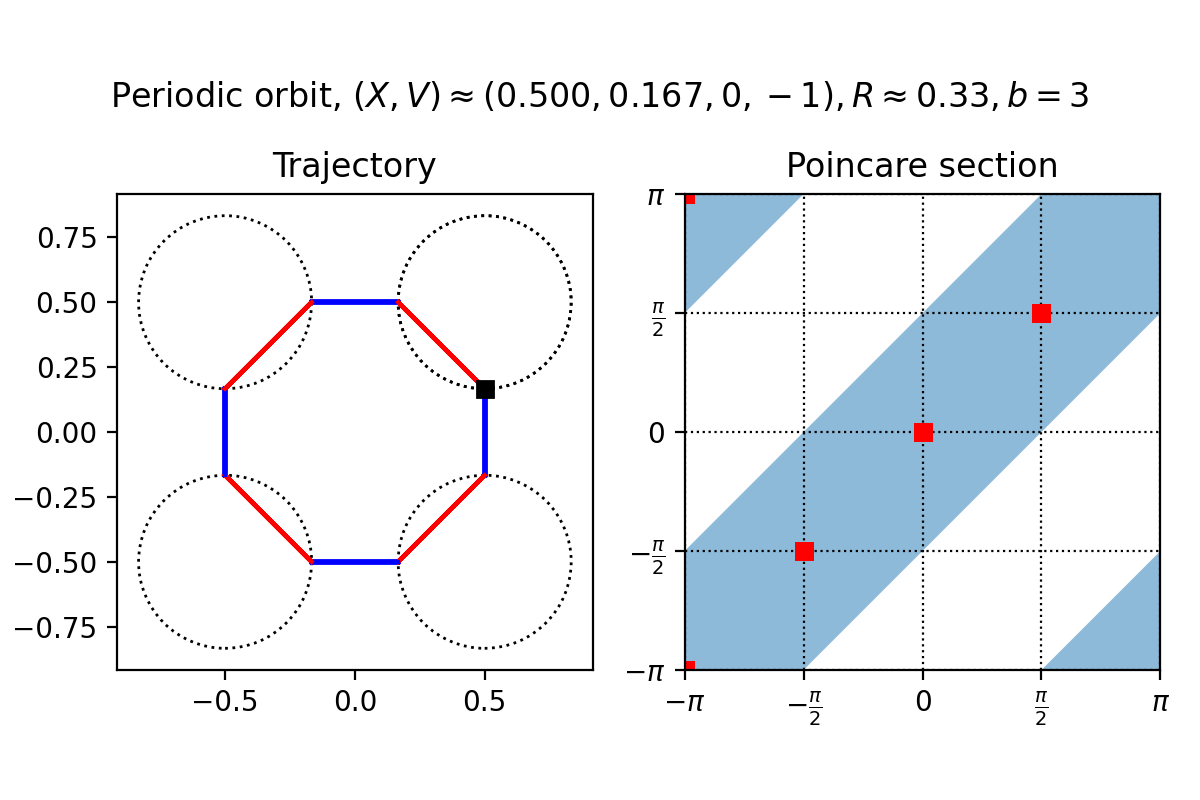
\includegraphics[width=\textwidth, trim={0 1cm 0 0cm}, clip]{stable_square_with_poincare.png}
\caption{}
\label{subfig:penandpaperorbits1}
\end{subfigure}
%
\begin{subfigure}{0.49\textwidth}
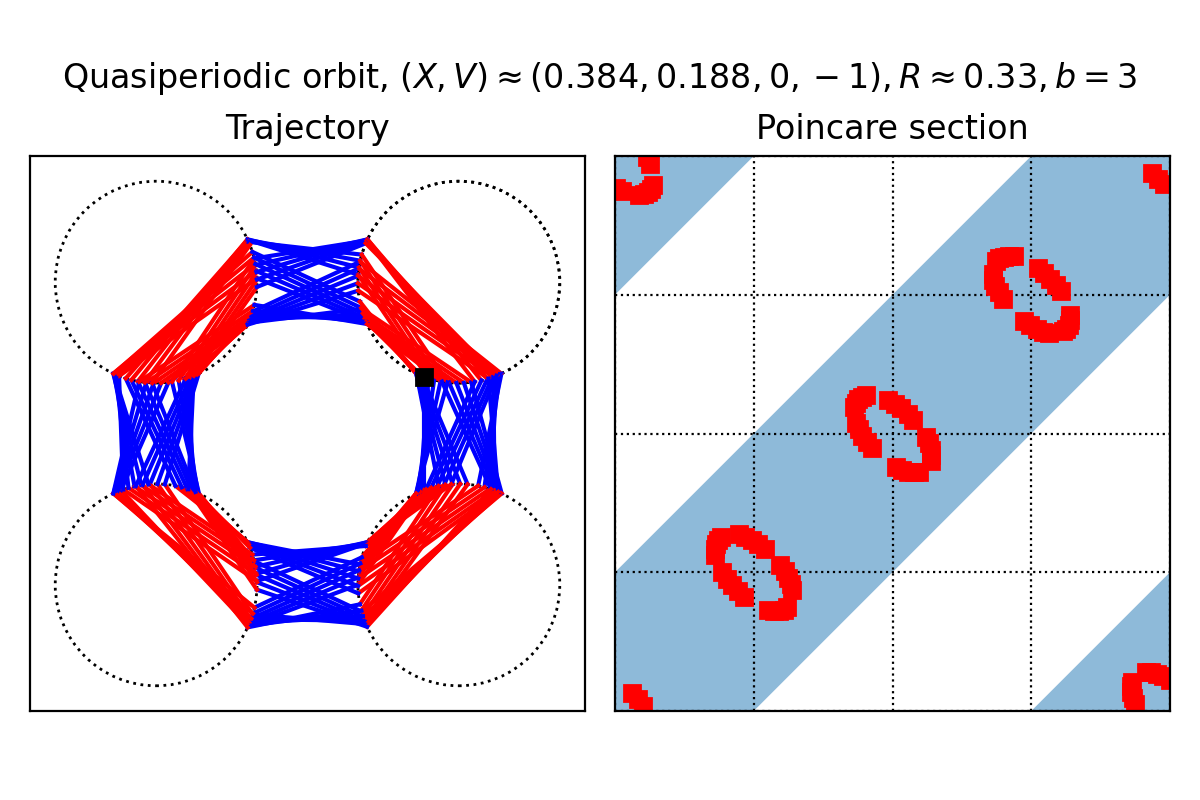
\includegraphics[width=\textwidth, trim={0 1cm 0 0cm}, clip]{perturbed_stable_square_with_poincare.png}
\caption{}
\label{subfig:penandpaperorbits2}
\end{subfigure}
\caption{Stable trajectories discovered analytically (more on next page).}
\end{figure}

\begin{figure}[!th]
\ContinuedFloat
\centering
\begin{subfigure}{0.49\textwidth}
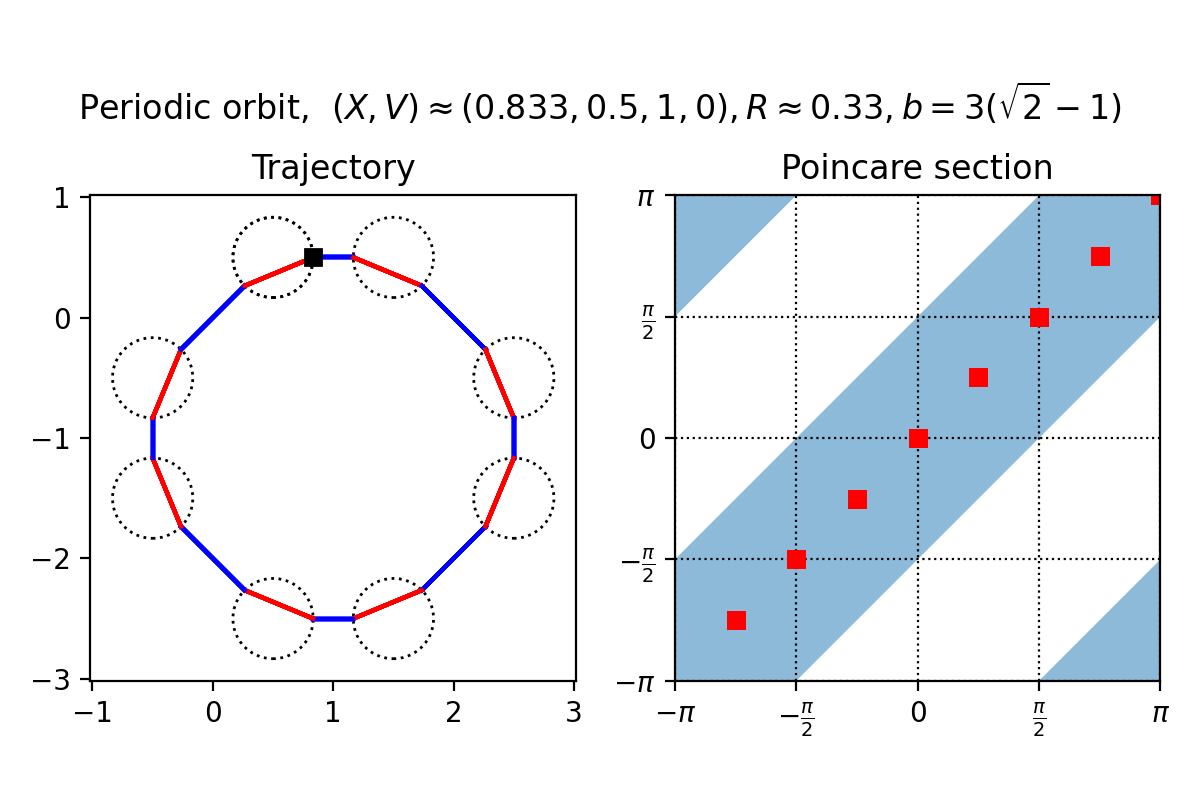
\includegraphics[width=\textwidth, trim={0 1cm 0 0cm}, clip]{stable_octagon_with_poincare.png}
\caption{}
\label{subfig:penandpaperorbits3}
\end{subfigure}
%
\begin{subfigure}{0.49\textwidth}
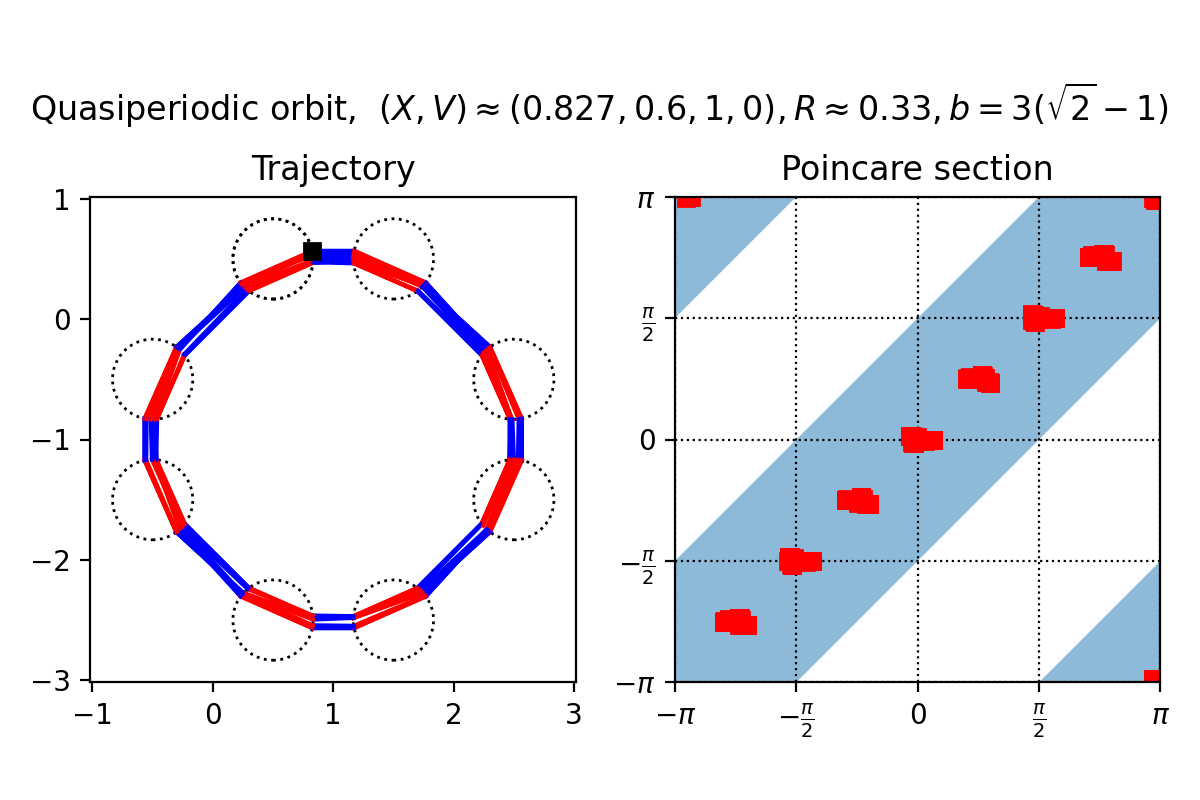
\includegraphics[width=\textwidth, trim={0 1cm 0 0cm}, clip]{perturbed_stable_octagon_with_poincare.png}
\caption{}
\label{subfig:penandpaperorbits4}
\end{subfigure}
%
\begin{subfigure}{0.49\textwidth}
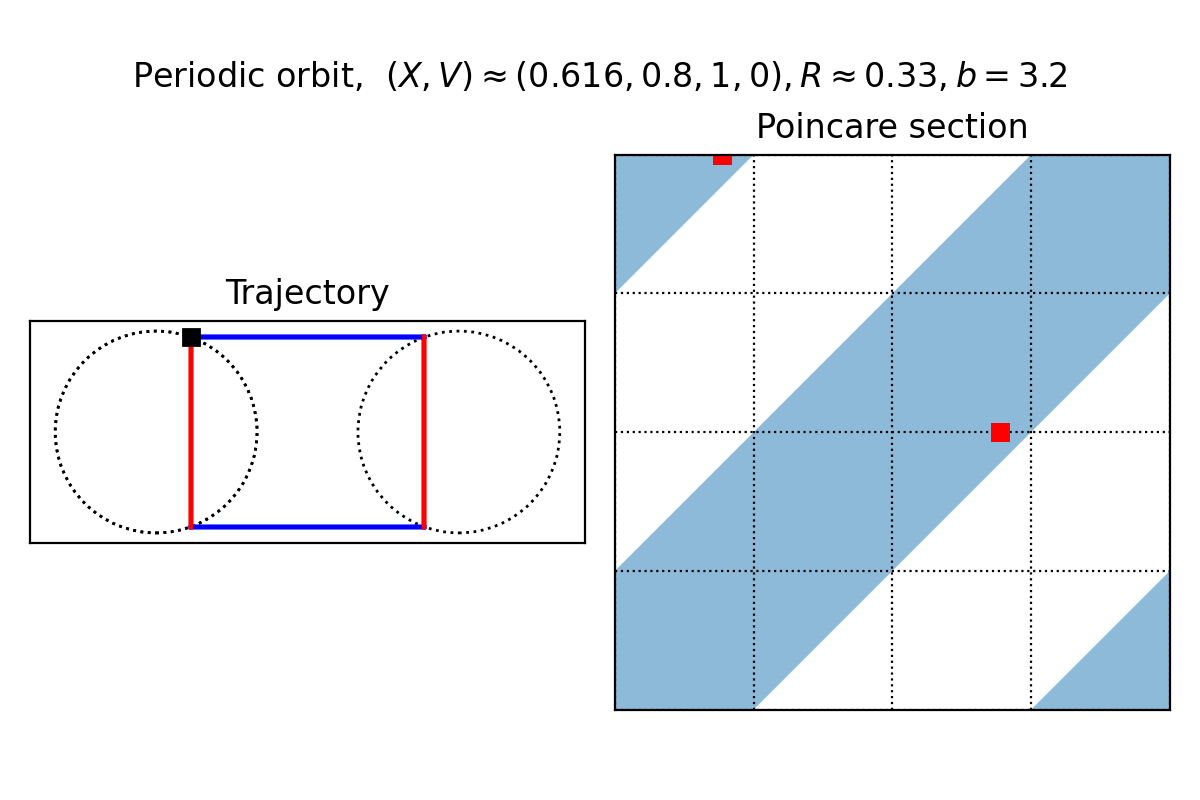
\includegraphics[width=\textwidth, trim={0 1cm 0 0cm}, clip]{unstable_square_with_poincare.png}
\caption{}
\label{subfig:penandpaperorbits5}
\end{subfigure}
%
\begin{subfigure}{0.49\textwidth}
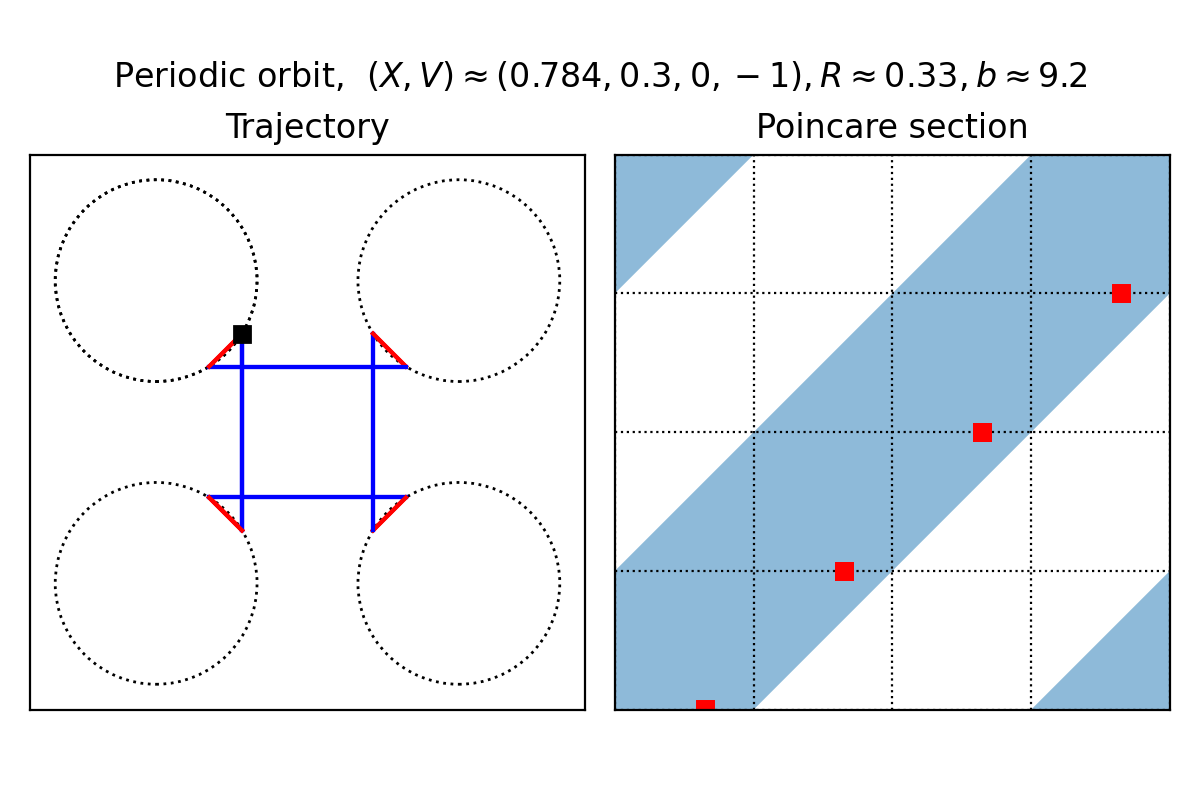
\includegraphics[width=\textwidth, trim={0 1cm 0 0cm}, clip]{unstable_loopy_square_with_poincare.png}
\caption{}
\label{subfig:penandpaperorbits6}
\end{subfigure}
\caption{Unstable trajectories discovered analytically.}
\label{fig:penandpaperorbits}
\end{figure}

The trajectories \cref{subfig:penandpaperorbits1}, \ref{subfig:penandpaperorbits3}, \ref{subfig:penandpaperorbits5}, and \ref{subfig:penandpaperorbits6} are periodic. \Cref{subfig:penandpaperorbits1} and \ref{subfig:penandpaperorbits3} are stable, \hl{we prove this in the python notebook [??]}, and \ref{subfig:penandpaperorbits2} and \ref{subfig:penandpaperorbits4} are given by perturbed initial conditions of each case, respectively. Meanwhile \ref{subfig:penandpaperorbits5}, \ref{subfig:penandpaperorbits6} are unstable, in fact, the plots are given only to 35 iterations due to sensitivity.

\begin{figure}[!th]
\centering
\begin{subfigure}{0.49\textwidth}
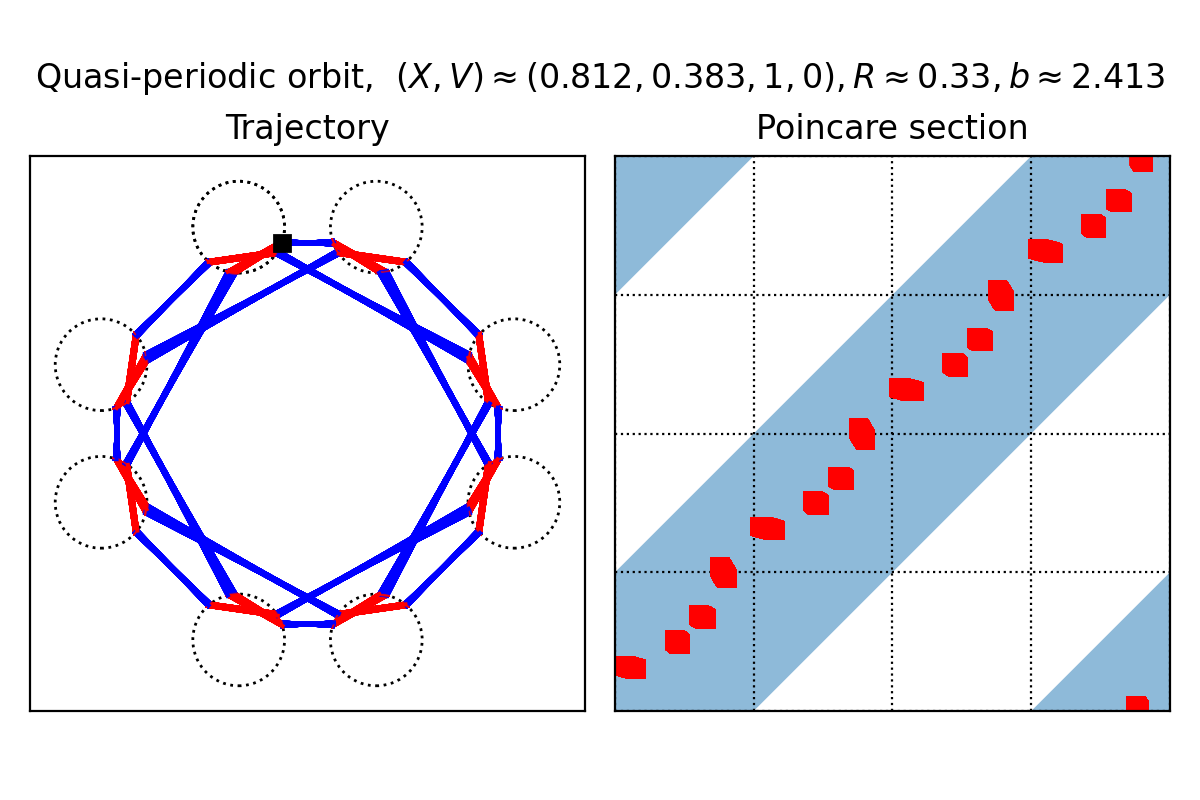
\includegraphics[width=\textwidth, trim={0 1cm 0 0cm}, clip]{star_with_poincare.png}
\caption{}
\label{subfig:star1}
\end{subfigure}
%
\begin{subfigure}{0.49\textwidth}
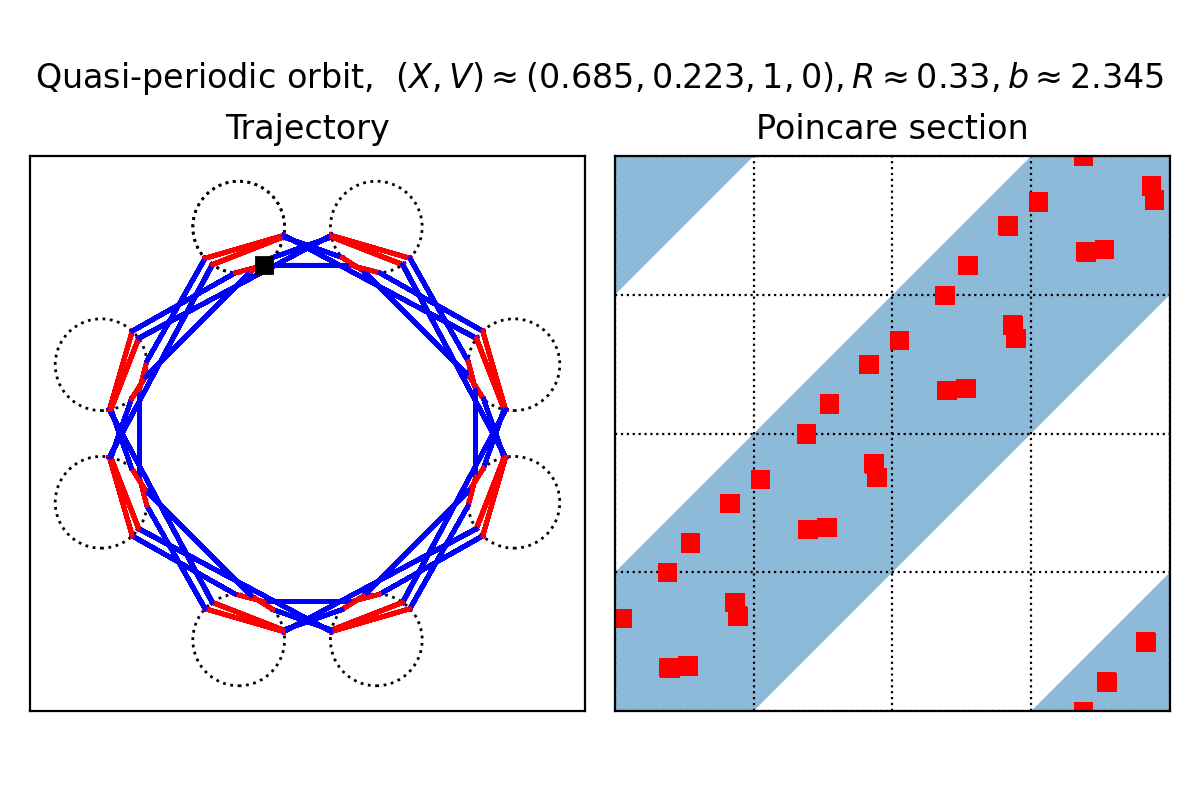
\includegraphics[width=\textwidth, trim={0 1cm 0 0cm}, clip]{doubled_star_with_poincare.png}
\caption{}
\label{subfig:star2}
\end{subfigure}
\caption{First signs of intricate quasi-periodicity.}
\label{fig:stars}
\end{figure}

\Cref{subfig:star1} and \ref{subfig:star2} are interesting, since they have a similar shape. The latter seems to be a ``doubled'' version of the former, and not a perturbation, since even after 2000 iterations the trajectory of \ref{subfig:star2} does not change, e.g., it does not smear like in the case of \ref{subfig:penandpaperorbits2}.

\begin{figure}[!th]
\centering
\begin{subfigure}{0.49\textwidth}
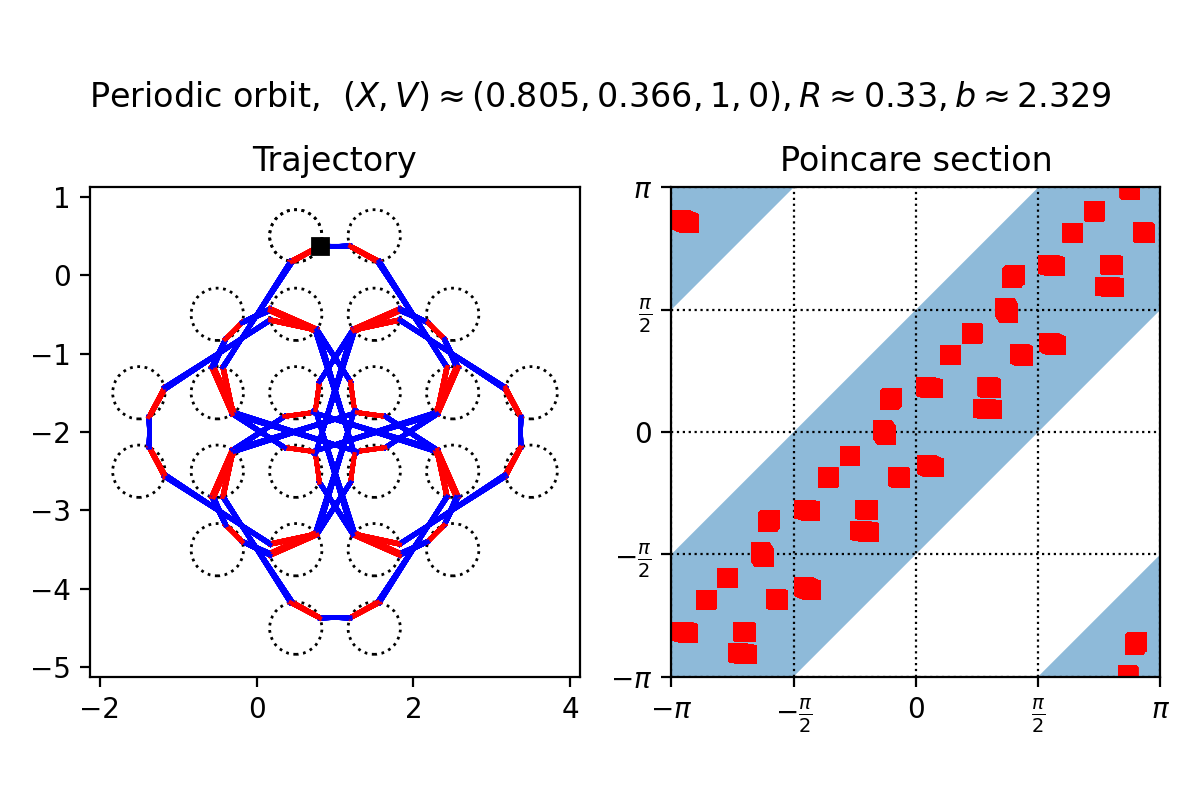
\includegraphics[width=\textwidth, trim={0 1cm 0 0cm}, clip]{sophisticated_with_poincare.png}
\caption{}
\label{subfig:ornamet1}
\end{subfigure}
%
\begin{subfigure}{0.49\textwidth}
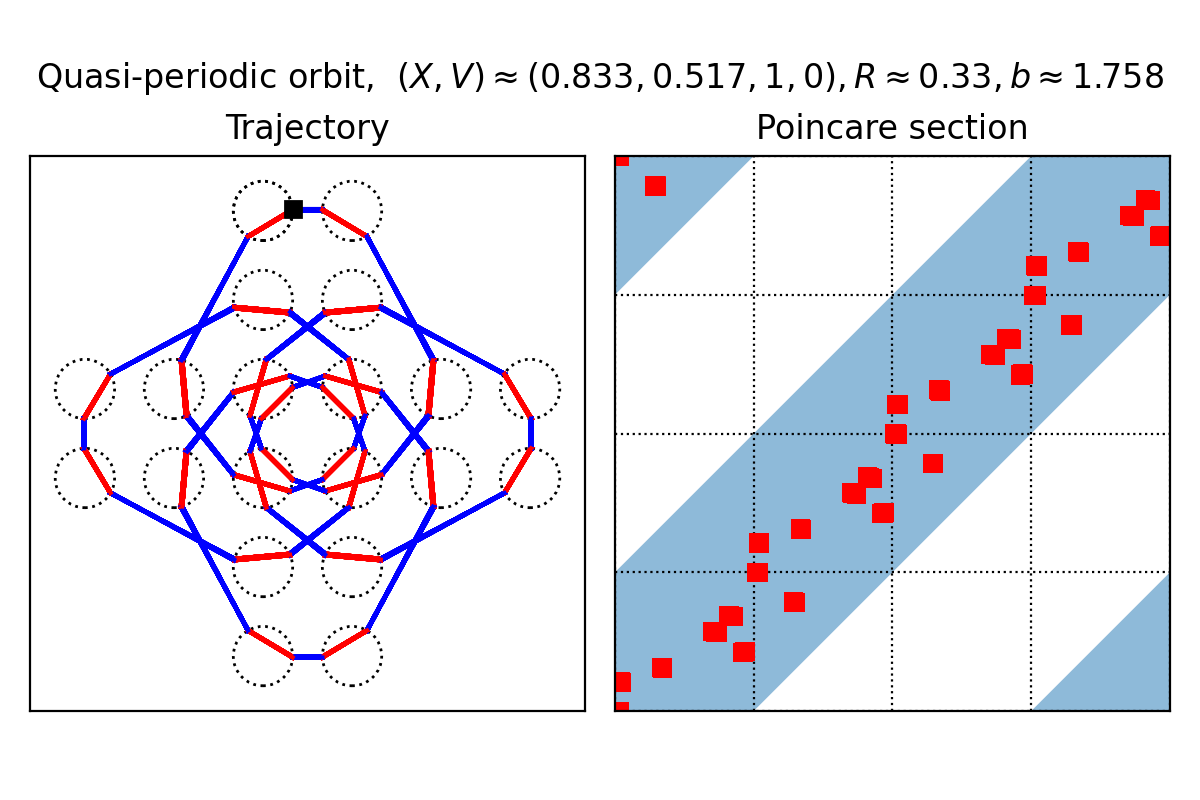
\includegraphics[width=\textwidth, trim={0 1cm 0 0cm}, clip]{distinguished_with_poincare.png}
\caption{}
\label{subfig:ornament2}
\end{subfigure}
\caption{Complex and ornamental quasi-periodic trajectories.}
\label{fig:ornaments}
\end{figure}

\newpage

\Cref{subfig:ornamet1} and \ref{subfig:ornament2} are surprisingly complex patterns, and unlike the rest of the examples, involve the most discs in the plane

\begin{figure}[!th]
\centering
\begin{subfigure}{0.49\textwidth}
\centering
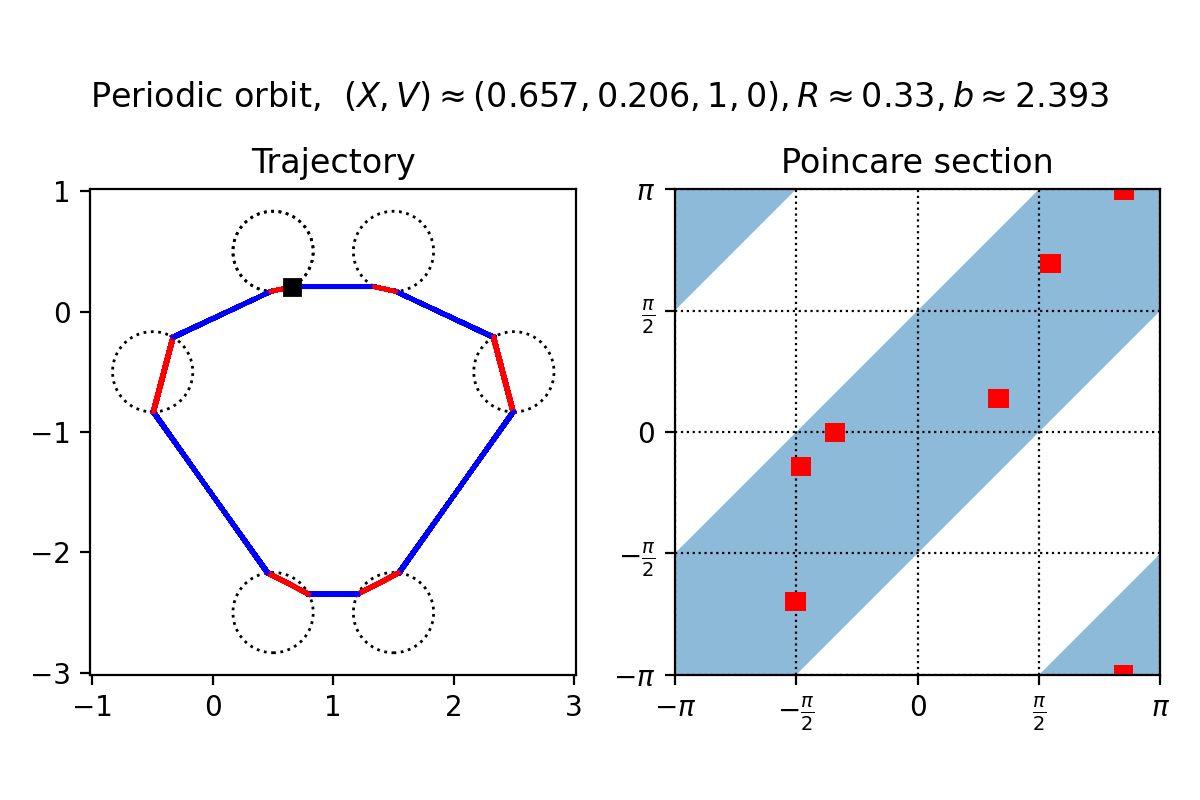
\includegraphics[width=\textwidth, trim={0 1cm 0 0cm}, clip]{lopsided_octagon_with_poincare.png}
\caption{}
\label{subfig:lopsidedhexagon}
\end{subfigure}
%
\begin{subfigure}{0.49\textwidth}
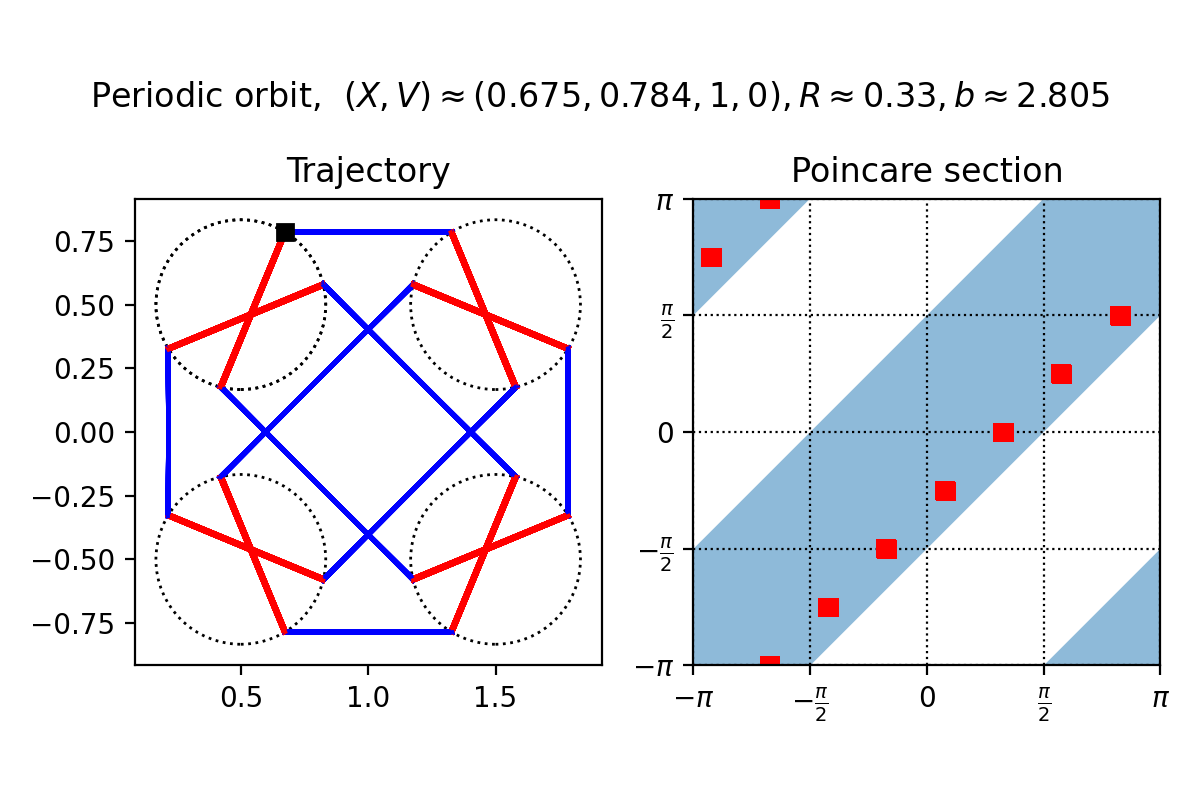
\includegraphics[width=\textwidth, trim={0 1cm 0 0cm}, clip]{strange_square_with_poincare.png}
\caption{}
\label{subfig:strangesquare}
\end{subfigure}
\caption{A symmetry breaking trajectory and an honorable mention.}
\label{fig:honorablementions}
\end{figure}

So far, we have seen trajectories that have square symmetries, the first to break this is \ref{subfig:lopsidedhexagon} with a bottom-heavy hexagon. It would be interesting to see if there are other polygon, for example triangles or pentagons. \Cref{subfig:strangesquare} does not illustrate anything new, we included it because it is aesthetically pleasing.

\begin{figure}[!th]
\centering
\begin{subfigure}{0.49\textwidth}
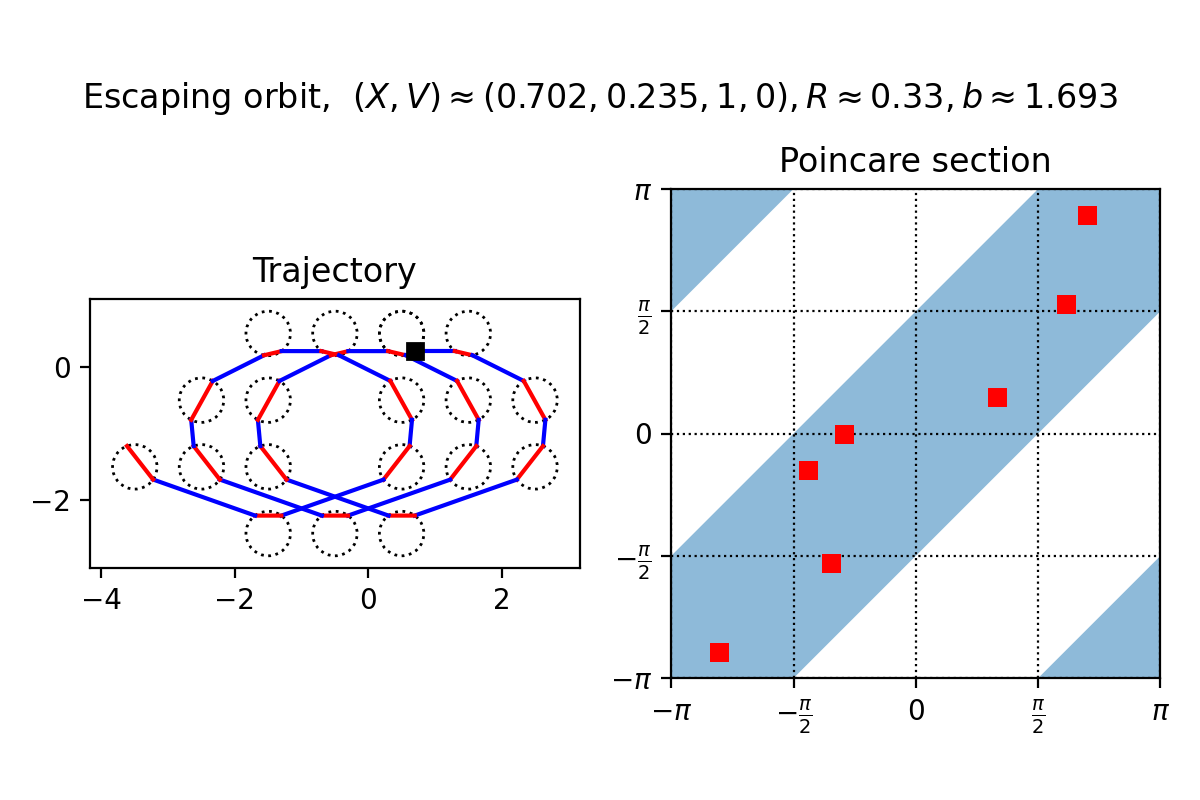
\includegraphics[width=\textwidth, trim={0 1cm 0 0cm}, clip]{walker_with_poincare.png}
\caption{}
\label{subfig:walker1}
\end{subfigure}
%
\begin{subfigure}{0.49\textwidth}
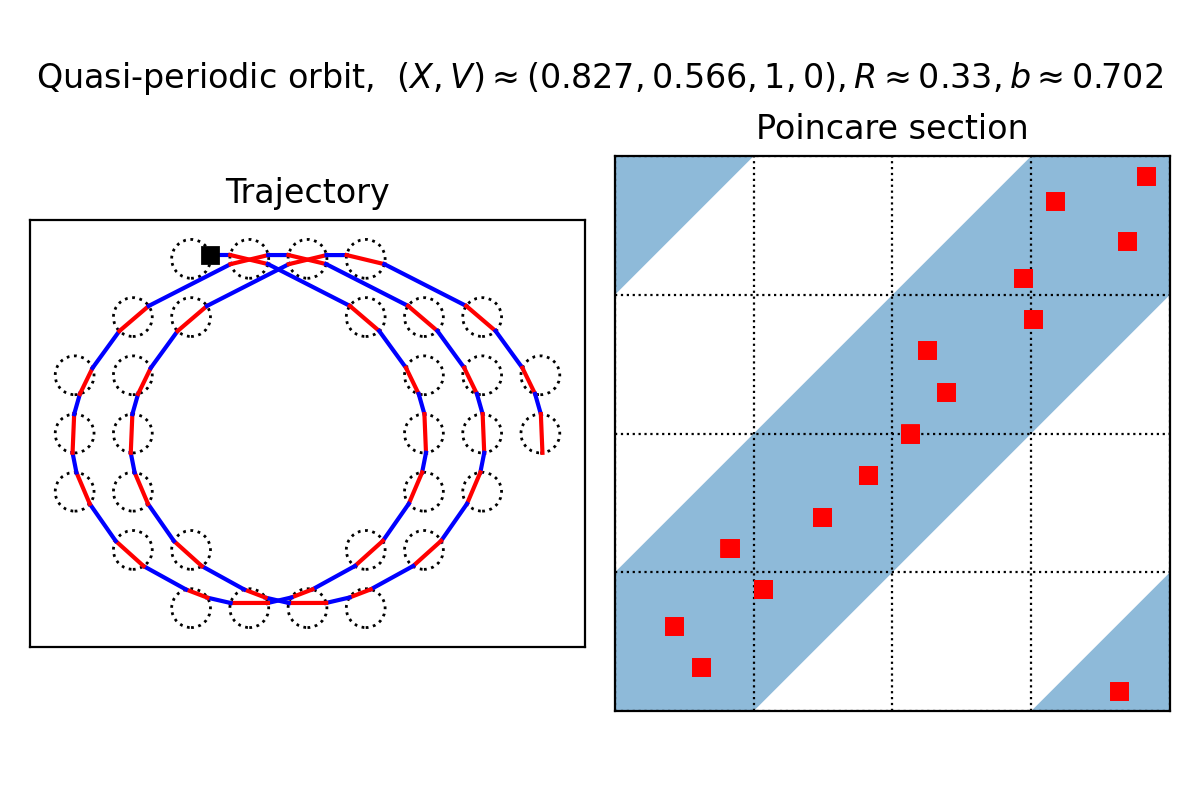
\includegraphics[width=\textwidth, trim={0 1cm 0 0cm}, clip]{big_walker_with_poincare.png}
\caption{}
\label{subfig:walker2}
\end{subfigure}
\caption{Wandering in $\mathbb R^2$, yet quasi-periodic in $\mathbb T$.}
\label{fig:walkers}
\end{figure}

In \cref{subfig:walker1} and \ref{subfig:walker2} we have the first examples of trajectories that wander in the plane but are quasi-periodic in the torus. It seems that these patterns arise in between values of $b$ that produce trajectories as in \cref{fig:bigcircles}, that is, as $b$ decreases, the radii of the circles in the pattern increases, and if, in a specific way, the circle does not close, you can still see repetition.

\begin{figure}[!th]
\centering
\begin{subfigure}{0.49\textwidth}
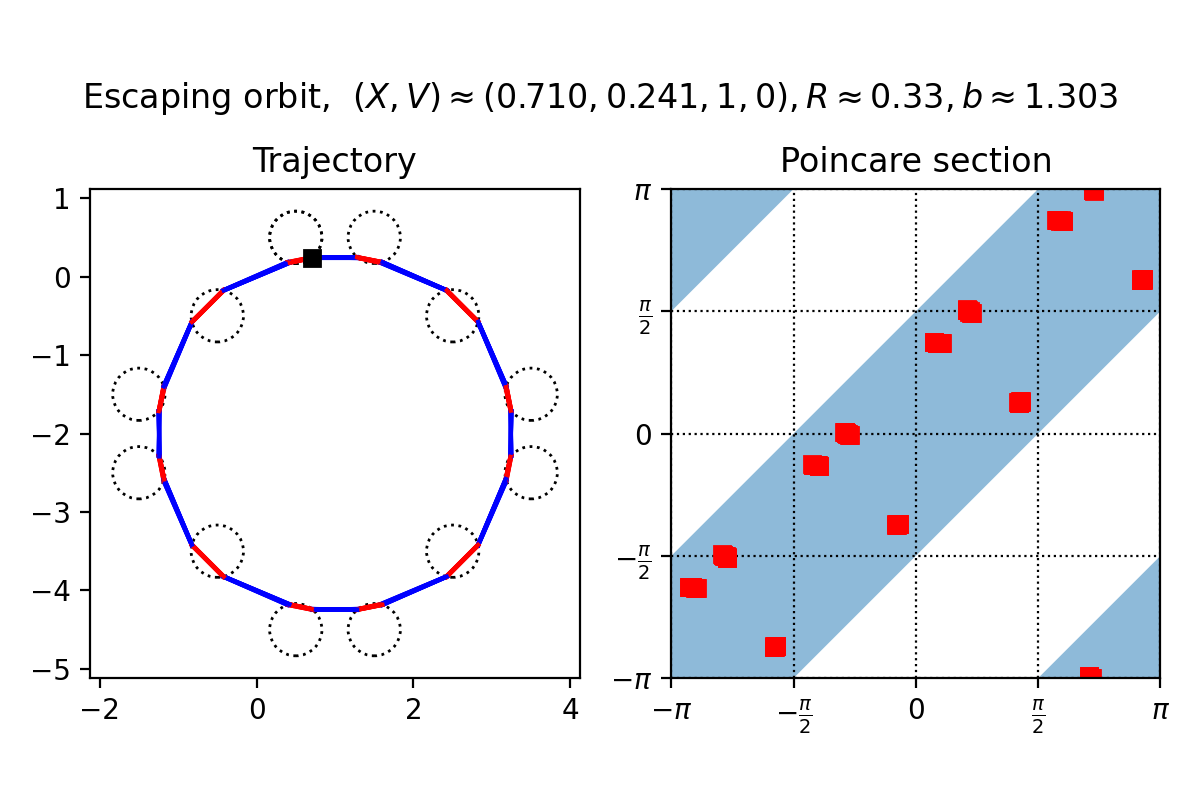
\includegraphics[width=\textwidth, trim={0 1cm 0 0cm}, clip]{12gon_with_poincare.png}
\caption{}
\label{subfig:bigcircle1}
\end{subfigure}
%
\begin{subfigure}{0.49\textwidth}
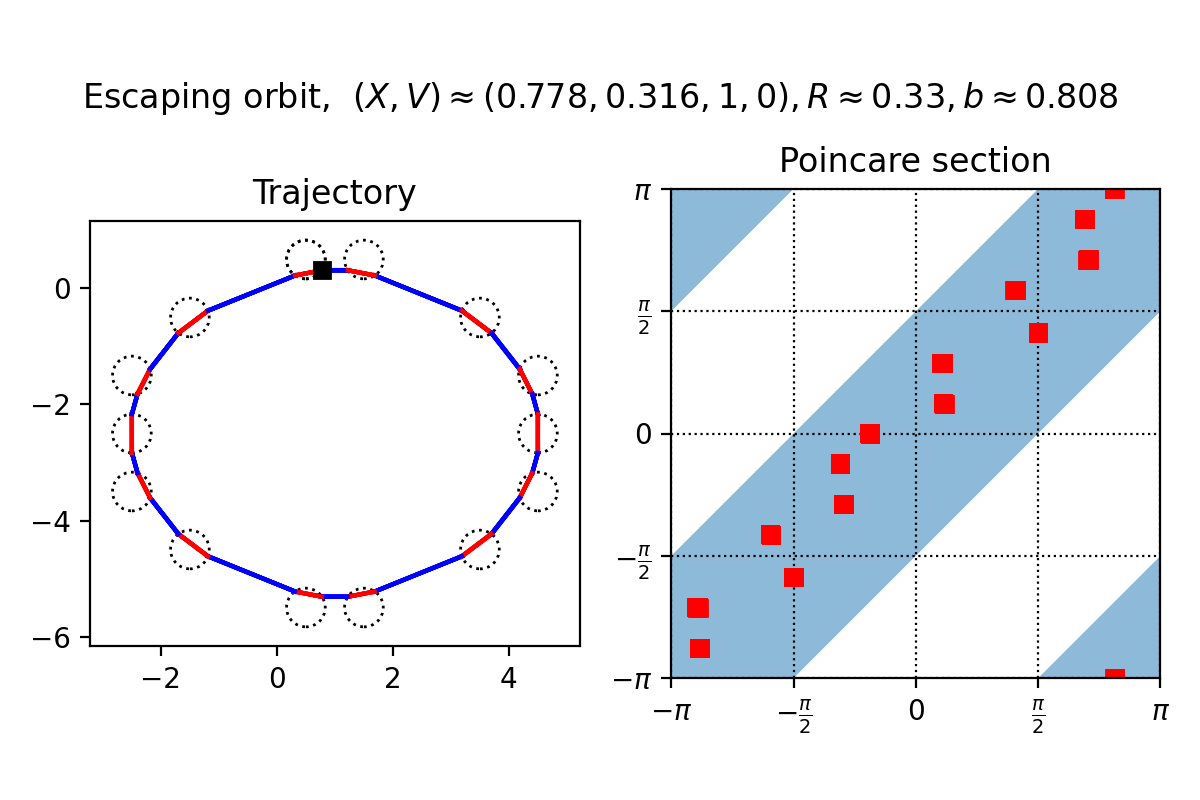
\includegraphics[width=\textwidth, trim={0 1cm 0 0cm}, clip]{egg_with_poincare.png}
\caption{}
\label{subfig:bigcircle2}
\end{subfigure}
%
\begin{subfigure}{0.49\textwidth}
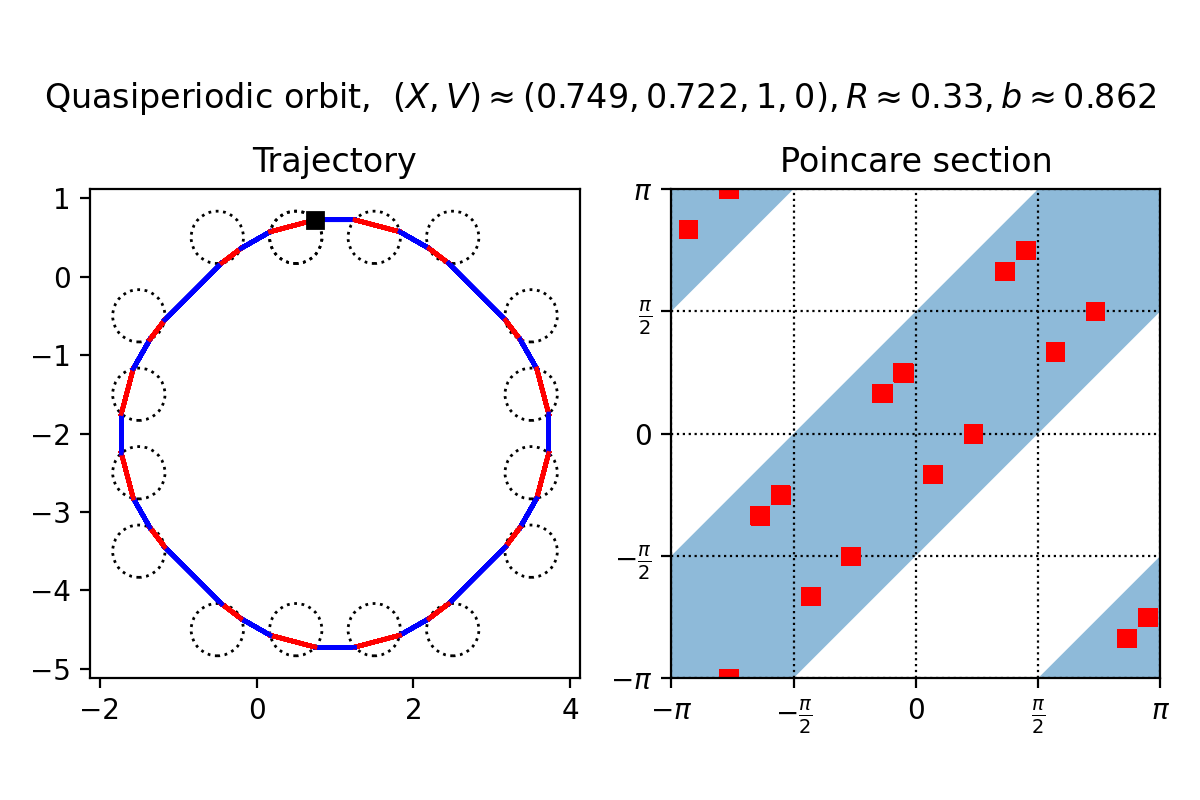
\includegraphics[width=\textwidth, trim={0 1cm 0 0cm}, clip]{big_square_with_poincare.png}
\caption{}
\label{subfig:bigcircle3}
\end{subfigure}
%
\begin{subfigure}{0.49\textwidth}
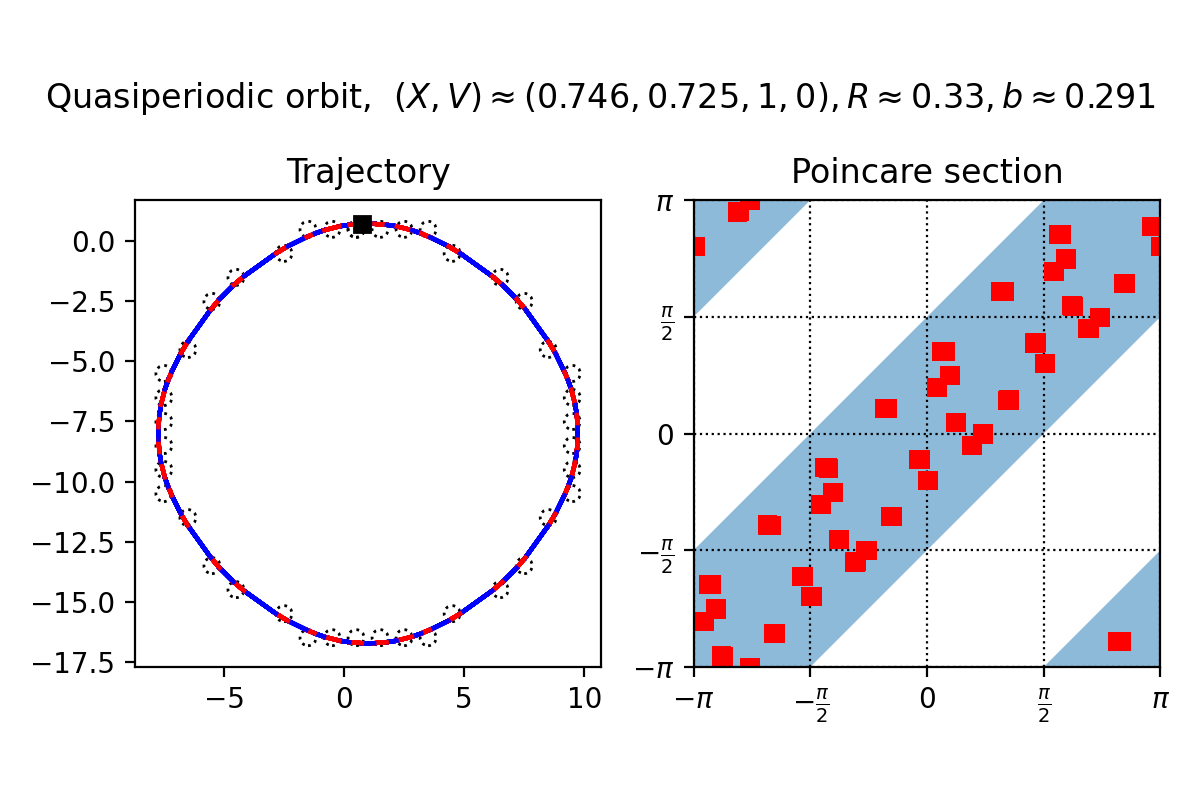
\includegraphics[width=\textwidth, trim={0 1cm 0 0cm}, clip]{big_circle_with_poincare.png}
\caption{}
\label{subfig:bigcircle4}
\end{subfigure}
\caption{Large circular trajectories for small values of $b$.}
\label{fig:bigcircles}
\end{figure}

The last \ref{subfig:bigcircle1} - \ref{subfig:bigcircle4} are examples with values of $b$ relatively small compared to the rest. The lower the value of $b$, the closer the shape resembles a circle, which is in line with what we had seen using KAM. We have not found any intricate patterns for low values of $b$.

We see that in this simple system there is interesting dynamics with varying levels of complexity. It is safe to say that at least some of these would be hard to find by hand, and would be feasible only with some numerics and a measure of complexity for determining good candidates. We now construct the Poincar\'e section $\Sin$ and after that we outline the methods we used to obtain these quasi-periodic trajectories.
